Figure~\ref{fig:temp} below visualizes how all the elements of the project are connected. All elements are built and run in Docker containers. This allows for the same result on every computer that runs these isolated containers. Providing all big components a separate container, allows for a more robust system. This simulates a real\hyp{}life scenario, by not having every object in the same container. In the real world, the onboard controller of the \acs{uav} is not in direct contact with for example a workstation nearby. This multi\hyp{}container environment communicates through a Docker network.

\begin{figure}[!h]
  \centering
  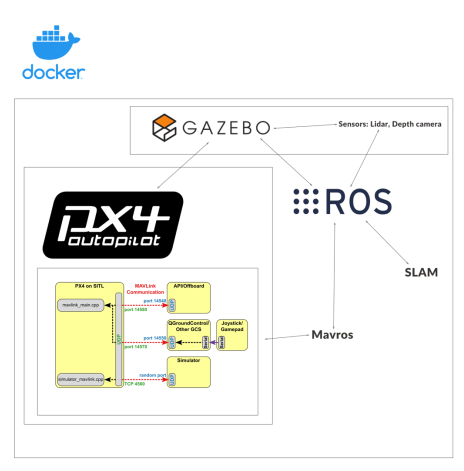
\includegraphics[width=0.6\linewidth]{temp.png}
  \caption{This is a temporary figure}
  \label{fig:temp}
\end{figure}